\documentclass{paper}

%\usepackage{times}
\usepackage{epsfig}
\usepackage{graphicx}
\usepackage{amsmath}
\usepackage{amssymb}
\usepackage{color}
\usepackage{caption}
\usepackage{subcaption}


% load package with ``framed'' and ``numbered'' option.
%\usepackage[framed,numbered,autolinebreaks,useliterate]{mcode}

% something NOT relevant to the usage of the package.
\setlength{\parindent}{0pt}
\setlength{\parskip}{18pt}
\graphicspath{{images/}}


\usepackage[latin1]{inputenc}
\usepackage[T1]{fontenc}


\usepackage{listings}
\lstset{%
   language=R,
   basicstyle=\small\ttfamily,
   frame=single
}



\title{Assignment 5}



\author{Jenni Simon\\09-116-005}
% //////////////////////////////////////////////////


\begin{document}



\maketitle


% Add figures:
%\begin{figure}[t]
%%\begin{center}
%\quad\quad   \includegraphics[width=1\linewidth]{ass2}
%%\end{center}
%
%\label{fig:performance}
%\end{figure}


\paragraph{Exercise 1}

Figure \ref{fig:res1} and listing \ref{list:res1} show results for the multiple
linear regression model with target variable "Wage".

As can be expected we observe that ID is not significant (high value for $P(>|t|)$) while
the other variables are clearly significant (very small $P(>|t|)$).
Looking at the t-values, we see that "Education" is the most
significant predictor (highest value for $|t|$). The residual plot in figure \ref{fig:res1} indicates that
the linear model fits the data quite well, given that the approximate mean (red line)
is close to zero and the variance of the residuals appears close to constant.
We observe that "Wage" increases with "Education" as well as being "Male". 

\begin{figure}
  \begin{center}
    \quad\quad
    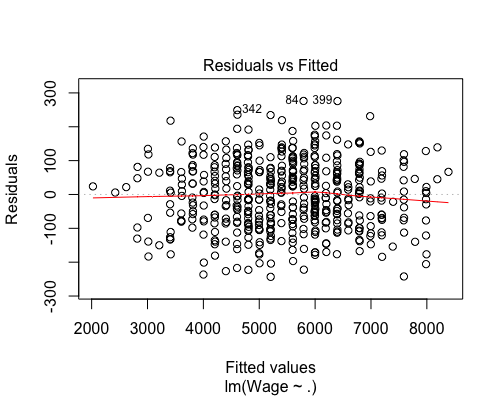
\includegraphics[width=.8\linewidth]{res1}
  \end{center}
  \caption{Plot showing the residuals against the fit of the multiple regression
   model of exercise 1.}
   \label{fig:res1}
\end{figure}

\begin{minipage}{\linewidth}
  \begin{lstlisting}[caption={Summary of multiple regression fit for exercise 1},
    label=list:res1]

Residuals:
     Min       1Q   Median       3Q      Max
-243.334  -75.119    2.669   70.007  276.238

Coefficients:
              Estimate Std. Error t value Pr(>|t|)
(Intercept) -576.22317   24.08079 -23.929   <2e-16 ***
ID             0.02952    0.03114   0.948    0.344
Education    397.90661    1.54440 257.645   <2e-16 ***
Gendermale   597.94707    9.17422  65.177   <2e-16 ***
---

Residual standard error: 100.1 on 493 degrees of freedom
Multiple R-squared:  0.9931,	Adjusted R-squared:  0.9931
F-statistic: 2.362e+04 on 3 and 493 DF,  p-value: < 2.2e-16

  \end{lstlisting}
\end{minipage}


\paragraph{Exercise 2}
Figure \ref{fig:res2} and listing \ref{list:res2} show results for the multiple
linear regression model with target variable 'PRP' after performing forward selection
for the variables to be included.

Forward selection was done by starting with an initial model using only an intersection
term and then adding variables one by one by finding the variable which decreases the RSS
the most. This is done for as long as the new model significantly reduces the RSS
measured using F-statistics.

By construction and looking at the included variables in listing \ref{list:res2} we
observe that given "MMAX", "CACH", "MMIN", "CHMAX" and "MYCT" the variables "MMIN"
and "CGMIN" are not significant in predicting "PRP". Also, "PRP"  increases with
all the included variables.

Figure \ref{fig:res2} also uncovers some quadratic behavior in the residual-plot
which is not captured by the purely linear model. Extending the model with some
quadratic terms would most probably lead to better results here.

\begin{figure}
  \begin{center}
    \quad\quad
    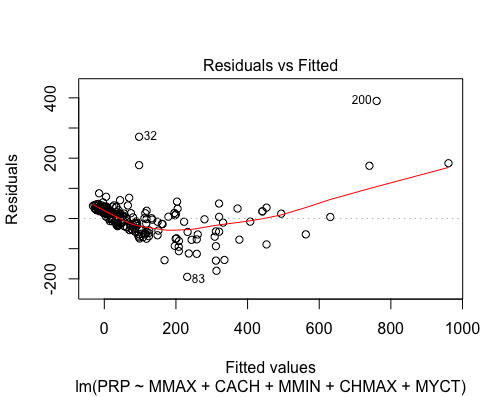
\includegraphics[width=.8\linewidth]{res2}
  \end{center}
  \caption{Plot showing the residuals against the fit of the multiple regression
   model of exercise 2.}
   \label{fig:res2}
\end{figure}

\begin{minipage}{\linewidth}
  \begin{lstlisting}[caption={Summary of multiple regression fit for exercise 2},
    label=list:res2]

Residuals:
    Min      1Q  Median      3Q     Max
-193.37  -24.95    5.76   26.64  389.66

Coefficients:
              Estimate Std. Error t value Pr(>|t|)
(Intercept) -5.608e+01  8.007e+00  -7.003 3.59e-11 ***
MMAX         5.562e-03  6.396e-04   8.695 1.18e-15 ***
CACH         6.298e-01  1.344e-01   4.687 5.07e-06 ***
MMIN         1.518e-02  1.788e-03   8.490 4.34e-15 ***
CHMAX        1.460e+00  2.076e-01   7.031 3.06e-11 ***
MYCT         4.911e-02  1.746e-02   2.813   0.0054 **
---

Residual standard error: 59.86 on 203 degrees of freedom
Multiple R-squared:  0.8648,	Adjusted R-squared:  0.8615
F-statistic: 259.7 on 5 and 203 DF,  p-value: < 2.2e-16

  \end{lstlisting}
\end{minipage}

\paragraph{Exercise 3}
The most important variable of the linear model of exercise 2 and also the first
variable added during forward selection is "MMAX". Figure \ref{fig:ex3} shows a
plot of the linear model using "MMAX" only against "PRP". We observe that the linear
model clearly underestimates at $MMAX=0$ and around $MMAX=6500$. This suggest that
probably a quadratic term $MMAX^2$ model would fit better.


\begin{figure}
  \begin{center}
    \quad\quad
    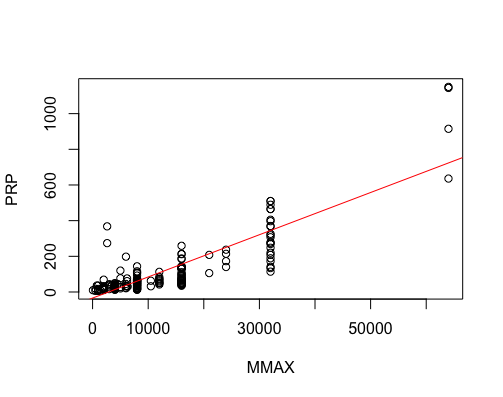
\includegraphics[width=.8\linewidth]{ex3}
  \end{center}
  \caption{Plot showing the linear regression
   model of exercise 3.}
   \label{fig:ex3}
\end{figure}

\paragraph{Exercise 4}

Figure \ref{fig:res4} and listing \ref{list:res4} show results for the multiple
linear regression model with target variable 'mpg' after performing forward selection
for the variables to be included.

By construction and looking at the included variables in listing \ref{list:res2} we
observe that given "weight", "year" and "origin" the variables "acceleration",
 "horsepower", "displacement" and "cylinders" are not significant in predicting
"mpg". Also, "mpg" increases with "year" and decreases with "weight". Supposing
that "origin" is a categorical variable with vales USA (1), Asia (3) or Europe (2),
USA has the lowest value of mpg followed by Europe and Asia.

Figure \ref{fig:res4} shows some non-linear behavior in the residual-plot
which is not captured by the linear model. Extending the model with some
higher order or interaction terms would most probably lead to better results.
We also observe some non-constant variance (i.e. heteroscedasticity?) in the data.

\begin{figure}
  \begin{center}
    \quad\quad
    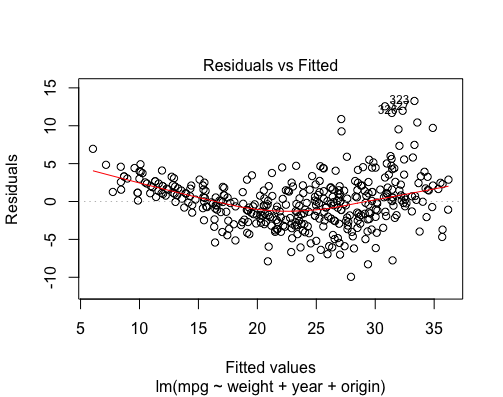
\includegraphics[width=.8\linewidth]{res4}
  \end{center}
  \caption{Plot showing the residuals against the fit of the multiple regression
   model of exercise 4.}
   \label{fig:res4}
\end{figure}

\begin{minipage}{\linewidth}
  \begin{lstlisting}[caption={Summary of multiple regression fit for exercise 4},
    label=list:res4]

Residuals:
    Min      1Q  Median      3Q     Max
-9.6025 -2.1132 -0.0206  1.7617 13.5261

Coefficients:
              Estimate Std. Error t value Pr(>|t|)
(Intercept) -1.831e+01  4.017e+00  -4.557 6.96e-06 ***
weight      -5.887e-03  2.599e-04 -22.647  < 2e-16 ***
year         7.698e-01  4.867e-02  15.818  < 2e-16 ***
origin2      1.976e+00  5.180e-01   3.815 0.000158 ***
origin3      2.215e+00  5.188e-01   4.268 2.48e-05 ***
---

Residual standard error: 3.337 on 387 degrees of freedom
Multiple R-squared:  0.819,	Adjusted R-squared:  0.8172
F-statistic: 437.9 on 4 and 387 DF,  p-value: < 2.2e-16

  \end{lstlisting}
\end{minipage}

The most important variable of the linear model  and also the first
variable added during forward selection is "weight". Figure \ref{fig:ex4} shows a
plot of the linear model using "weight" only against "mpg". We again observe that
the model tends to underestimate at the borders and overestimate in the middle.
Probably a quadratic term $weight^2$ would give a better fit.

\begin{figure}
  \begin{center}
    \quad\quad
    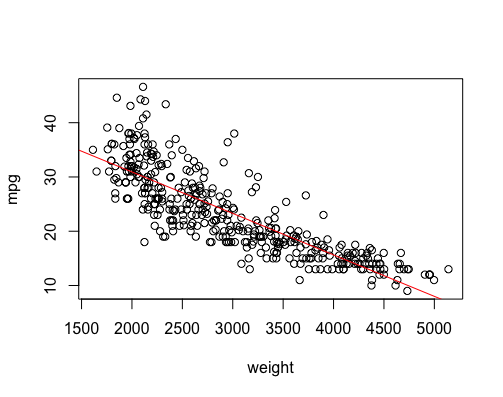
\includegraphics[width=.8\linewidth]{ex4}
  \end{center}
  \caption{Plot showing the linear regression
   model of exercise 4.}
   \label{fig:ex4}
\end{figure}


\end{document}
